
\documentclass[12pt,onecolumn]{article}
\usepackage[brazilian]{babel}
\usepackage[utf8]{inputenc}
\usepackage{hyperref}
\usepackage[section]{placeins}
\usepackage{graphicx}
\usepackage{caption}
\usepackage{subcaption}
\usepackage{float}
\usepackage{framed,color}

\begin{document}

% Title page.
\begin{titlepage}

    % Title info.
    \title{
        \bf
        \LARGE Apostila de \\
        \Huge  Gimp
    }
    
    \author{Renan Teruo Carneiro \\ Wilson Kazuo Mizutani}
    
    % Print title.
    \maketitle
    
    % No numbering on this page.
    \thispagestyle{empty}
    
\end{titlepage}

% Print table of contents.
\tableofcontents

% Page break.
\clearpage

\section{Sobre o Gimp}
  O Gimp é legal.

\section{Instalando}
  Baixa e clique avançar-avançar-indução seja feliz.
  Ou sudo apt-get install.

\section{Introdução}
  Como uma introdução ao Gimp, vamos fazer uma edição bem simples. O objetivo
  será colorir a imagem de um ícone preto-e-branco, como mostrado na Figura
  \ref{fig:intro}. A imagem original está disponível em
  
  \begin{center}
    \url{http://game-icons.net/lorc/original/beast-eye.html}      
  \end{center}
  
   O ideal é pegar a versão com maior resolução possível, em PNG.

  \begin{figure}
  \centering
  \begin{subfigure}{.5\textwidth}
    \centering
    
\includegraphics[width=.7\linewidth]{beast-eye.png}
    \label{fig:ex1_before}
  \end{subfigure}%
  \begin{subfigure}{.5\textwidth}
    \centering
    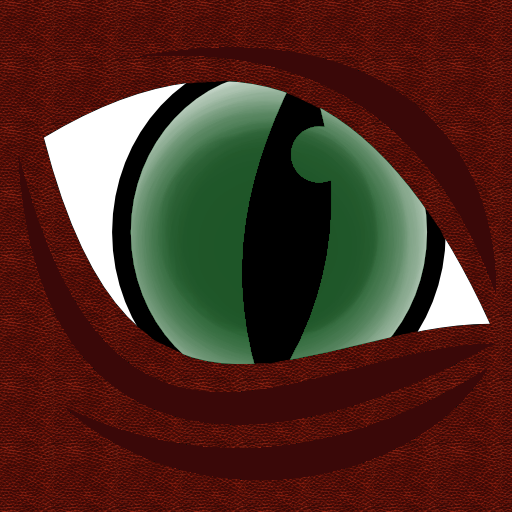
\includegraphics[width=.7\linewidth]{draft00.png}
    \label{fig:ex1_after}
  \end{subfigure}
  \caption{
    \footnotesize
    \it
    Imagem antes e depois da edição
  }
  \label{fig:intro}
  \end{figure}
  
  Com esse exercício esperamos apresentar as funcionalidades básicas e as
  técnicas essenciais para se manipular imagens com o Gimp. Mas apesar do foco
  nesse momento ser passar os conceitos básicos para o aluno, também
  introduziremos algumas das principais ferramentas usadas em projetos Gimp.
  
  \subsection{Abrindo a imagem e convertendo para RGBA}
    O primeiro passo do exercício é dizer para o Gimp que queremos trabalhar em
    RGBA (isso é, com cores e transparência) ao invés de Grayscale, que é o
    formato no qual a imagem do ícone está. E vamos aproveitar esse passo para
    mostrar o básico de copiar e colar imagens com Gimp (que não é muito
    diferente do convencional).
    
    Começamos abrindo a imagem original indo em {\bf File $\rightarrow$ Open}
    ou digitando {\bf CTRL+O}.
    
    \begin{framed}
      Algo que facilita muito o uso do Gimp é a familiarização com os atalhos
      de teclado. Saber uma meia-dúzia de atalhos é o suficiente para tornar
      dobrar a eficiência de trabalho. 
    \end{framed}
    
    Do jeito que o Gimp carrega a imagem (em Grayscale) não é possível aplicar
    nenhuma cor aos pixeis. Isso significa que se selecionarmos, por exemplo,
    a {\bf Pencil Tool} (atalho {\bf N}), e mudarmos a cor para vermelho, ainda
    assim pintaremos apenas tons de cinza.
    
    \begin{figure}[h]
      \centering
      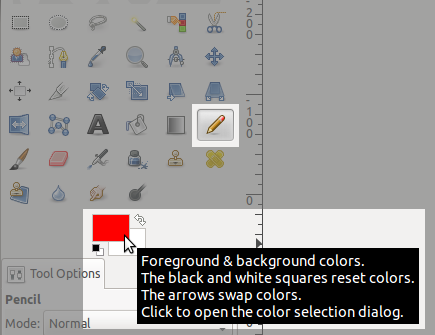
\includegraphics[width=.6\textwidth]{screenshots/00-pencil_and_color.png}
      \caption{
        \footnotesize
        \it
        Seleciondo a {\bf Pencil Tool} e mudando a cor.
      }
      \label{fig:pencil_and_color}
    \end{figure}
    
    \begin{framed}
      Para mudar de cor no Gimp, basta clicar duas vezes no retângulo colorido
      no meio da {\bf Toolbox }, como mostra a Figura \ref{fig:pencil_and_color}.
    \end{framed}
    
    \begin{framed}
      Para desfazer uma ação Gimp, pode-se ir em {\bf Edit $\rightarrow$ Undo}
      ou digitar {\bf CTRL+Z}. É um comando {\it extremamente útil}, e o
      histórico de ações que o Gimp guarda é bastante grande. Use ele para
      desfazer quaisquer alterações que você possa ter feito na imagem original
      antes de seguir os próximos passos.
    \end{framed}
    
    Vamos, então, criar uma nova imagem que use RGBA ao invés de Grayscale. Para
    isso, clicamos em {\bf File $\rightarrow$ New} ou digitamos {\bf CTRL+N}. Um
    menu {\bf Create a New Image} aparecerá. Nele temos acesso à várias
    configurações da nova imagem, como a largura e a altura dela. Essas
    manteremos como estão (512x512 se você pegou a maior resolução disponível).
    O que nos interessa aqui é mudar o formato de cores e o suporte a
    transparência. Basta mudar essas configurações conforme a Figura
    \ref{fig:grayscale_to_RGBA}.
    
    \begin{figure}[H]
      \centering
      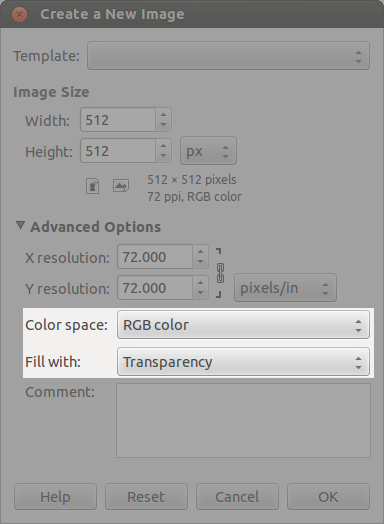
\includegraphics[scale=.55]{screenshots/00-grayscale_to_RGBA.png}
      \caption{
        \footnotesize
        \it
        Criando uma imagem RGBA
      }
      \label{fig:grayscale_to_RGBA}
    \end{figure}
    
    Uma vez feito isso, basta voltarmos para a imagem original, e:
    
    \begin{itemize}
      \item
        Selecionarmos ela inteira com {\bf Botão Direito do Mouse $\rightarrow$
        Selection $\rightarrow$ All} ou {\bf CTRL+A}.
      \item
        Copiarmos ela com {\bf Botão Direito do Mouse $\rightarrow$ Edit
        $\rightarrow$ Copy} ou {\bf CTRL+C}.
      \item
        Voltarmos para a imagem com RGBA que acabamos de criar.
      \item
        Colarmos o ícone orignal nela com {\bf Botão Direito do Mouse
        $\rightarrow$ Edit $\rightarrow$ Paste} ou {\bf CTRL+V}.
    \end{itemize}
    
    
  \subsection{Sobre seleções}
    Agora que temos nossa imagem pronta para ser manipulada, vamos falar sobre
    seleções no Gimp. Seleções são um conceito primordial para qualquer tipo de
    edição, pois {\bf toda ferramenta que não seja de seleção, só é aplicada
    sobre a seleção atual}. Quando não há nenhuma seleção, então a imagem toda
    é considerada selecionada (ou seja, as ferramentas serão aplicadas em todas
    as partes dela).
    
    Para entender isso melhor, podemos escollher a {\bf Rectangle Selection
    Tool} (atalho {\bf R}) e selecionar uma região qualquer da imagem
    clicando e arrastando o mouse, e depois soltando-o. Agora, se escolhermos,
    por exemplo, a {\bf Bucket Feel Tool} (atalho {\bf SHIFT+B}) e tentarmos
    usá-la, obteremos o resultado mostrado na Figura
    \ref{fig:selective_painting}.
  
    \begin{figure}[H]
      \centering
      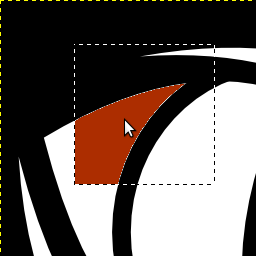
\includegraphics[scale=0.6]{screenshots/01-selective_painting.png}
      \caption{
        \footnotesize
        \it
        As ferramentas trabalham apenas nas regiões selecionadas
      }
      \label{fig:selective_painting}
    \end{figure}
    
    Outras duas ferramentas de seleção que vamos usar bastante são a {\bf
    Free Select Tool} (atalho {\bf F}) e a {\bf Fuzzy Select Tool} (atalho
    {\bf U}). A primeira permite selecionar uma região à mão livre e a segunda
    seleciona uma região que tenha uma cor em comum. Recomendamos experimentar
    um pouco com ela antes de prosseguir. Possíveis resultados do uso dessas
    ferramentas podem ser vistas na Figura \ref{fig:select_tools}.
    
    \begin{figure}[h]
      \centering
      \begin{subfigure}{.5\textwidth}
        \centering
        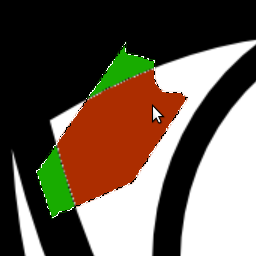
\includegraphics[width=.7\linewidth]{screenshots/02-free_select.png}
        \label{fig:free_select}
      \end{subfigure}%
      \begin{subfigure}{.5\textwidth}
        \centering
        
\includegraphics[width=.7\linewidth]{screenshots/03-fuzzy_select.png}
        \label{fig:fuzzy_select}
      \end{subfigure}
      \caption{
        \footnotesize
        \it
        Free Select Tool (esquerda) e Fuzzy Select Tool (direita).
      }
      \label{fig:select_tools}
    \end{figure}
    
    \begin{framed}
      A {\bf Free Select Tool} também pode ser usada traçando retas. Cada ponto
      que você clicar será ligado ao anterior, até que você volte a clicar no
      primeiro. Então, a região será selecionada. Também é possível misturar
      trechos retos e à mão livre.
    \end{framed}
  
    Agora, vamos afazer algo mais útil. Vamos colorir a pupila do olho na
    imagem. Como é de se esperar, para isso precisamos selecionar a pupila. A
    primeira ideia é usar a {\bf Fuzzy Selection Tool} e clicar nas regiões que
    correspondem à pupila. No entanto, como nas bordas dessa região há uma
    transição do branco para o preto, a seleção não fica perfeita (partes da
    borda ficam de fora). Além disso, mesmo que selecionássemos um dos lados da
    pupila, como selecionar o outro ao mesmo tempo?
    
    \begin{figure}[h]
      \centering
      
\includegraphics[width=.5\textwidth]{screenshots/04-pupil.png}
      \caption{
        \footnotesize
        \it
        O objetivo é selecionar apenas a pupila para podermos manipulá-la sem
        correr o risco de "vazar" para as outras partes da imagem
      }
      \label{fig:pupil}
    \end{figure}
    
    É nesse ponto que entram as {\bf operações de seleção}. Começando pelo
    primeiro problema, o grande obstáculo é que a {\bf Fuzzy Selection Tool} não
    alcança todas as partes da região branca, isso é, fica {\it faltando pixels}
    na região selecionada e {\it sobrando} na região não selecionada. Por outro
    lado, o mesmo acontece se a usamos para selecionar a região preta. Então uma
    plausível solução seria pegarmos o {\it inverso} da região preta. A {\bf
    operação de inversão} é a primeira das operações de seleção, e pode ser
    realizada usando {\bf Botão Direito do Mouse $\rightarrow$ Select
    $\rightarrow$ Invert} ou {\bf CTRL+I}.
    
    Mas então temos outro problema: todas as regiões brancas ficaram
    selecionadas. Para resolver isso usamos a {\bf operação de intersecção} ou
    a {\bf operação de diferença}. Diferentemente da operação de inversão, essas
    operações são aplicadas com o auxílio de alguma ferramenta de seleção. No
    caso, vamos usar a {\bf Free Select Tool}.
    
    Para ativar a operação de intersecçao, basta segurar {\bf CTRL+SHIFT} e usar
    a ferramenta de seleção. Quando terminar, {\bf todas as regiões em comum}
    entre a região até então selecionada e a nova comporão a nova seleção.
    
    Para ativar a operação de diferença, deve-se segurar {\bf CTRL} e usar a
    ferramenta de seleção. No final, as novas regiões selecionadas serão {\bf
    subtraídas} da seleção antiga.
    
    \begin{framed}
      A última operação de seleção é a {\bf operação de soma}. Ela é ativada
      segurando {\bf SHIFT} antes de usar uma ferramenta de seleção, e a nova
      região selecionada é somada à que havia antes.
    \end{framed}
    
    \begin{figure}[h]
      \centering
      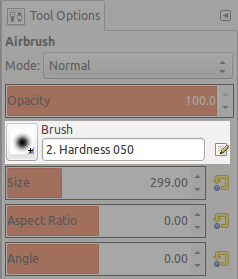
\includegraphics[width=.5\textwidth]{screenshots/04-setting_brush.png}
      \caption{
        \footnotesize
        \it
        Muda-se o pincel ({\it brush}) usado por uma ferramenta de manipulação
        na região destacada.
      }
      \label{fig:setting_brush}
    \end{figure}
    
    Quando, enfim, a pupila estiver devidamente selecionada, use alguma
    ferramenta de manipulação para deixá-la como preferir. No nosso exemplo,
    usamos a {\bf Airbrush Tool}. Ajustamos o formato do pincel dela na opção
    indicada na Figura \ref{fig:setting_brush}, e aumentamos seu tamanho até
    ficar do tamanho da pupila. Por fim, aplicamos ela no centro da pupila (que,
    em particular, não está na região selecionada) e obtivemos o resultado da
    Figura \ref{fig:pupil}.
    
    \begin{framed}
      Para aumentar ou diminuir o tamanho de uma ferramenta de manipulação,
      usa-se os botões {\bf \verb$[$} e {\bf \verb$]$}, respectivamente.
    \end{framed}
    
    Uma dificuldade comum quando se começa a usar o Gimp é saber como mover
    seleções. Quando tentamos mover uma região selecionada usando a {\bf Move
    Tool}, por exemplo, apenas o contorno da região se move, e não o conteúdo
    dela. Para fazer isso, é preciso recortar e logo em seguida colar de volta a
    região selecionada. Só então é que a região junto com seu conteúdo poderá
    ser movida.
    
    \begin{framed}
      Para recortar podemos usar {\bf Botão Direito do Mouse $\rightarrow$ Edit
      $\rightarrow$ Cut} ou o atalho {\bf CTRL+X}.
    \end{framed}
    
    %% 5) Mencionar como mover seleções.
        
  \subsection{Sobre camadas}
    %% 1) Vamos fazer uma camada para o olho. Selecione apenas o olho.
    %% 2) CTRL+X, CTR+V, colar em nova camada.
    \begin{figure}[H]
      \centering
      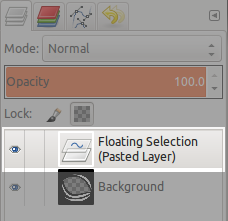
\includegraphics[width=.5\textwidth]{screenshots/05-pasted_layer.png}
      \caption{Seleções coladas ficam em uma camada flutuante}
      \label{fig:pasted_layer}
    \end{figure}
    %% 3) Camadas 101
    %% 4) Renomear camada nova (F2 ou "Edit Layer Attributes")
    %% 5) Redimensionar camada para o tamanho da imagem
    %% 6) Preencher o vazio na camada de baixo (usar balde)
    %% 7) Separar as estrias em outra camada também.
    \begin{figure}[H]
      \centering
      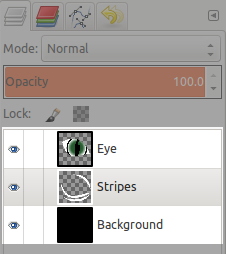
\includegraphics[width=.5\textwidth]{screenshots/07-layers.png}
      \caption{As três camadas no final}
      \label{fig:layers}
    \end{figure}
    
  \subsection{Finalizando}
    %% 1) Pintar as estrias (explicar o modo "fill selection" do balde)
    \begin{figure}[H]
      \centering
      
\includegraphics[width=.5\textwidth]{screenshots/06-partial.png}
      \caption{Resultado quase pronto da edição}
      \label{fig:partial}
    \end{figure}
    %% 2) Preencher o fundo com a textura "Leather" usando balde.
    %% 3) Ajustar cores, tons, etc.
    \begin{figure}[H]
      \centering
      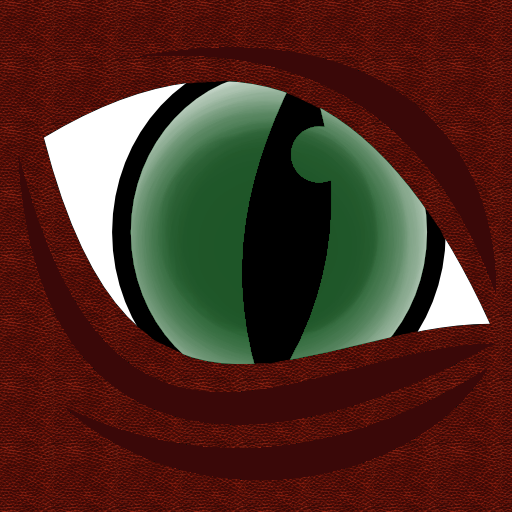
\includegraphics[width=.7\linewidth]{draft00.png}
      \caption{Resultado final}
      \label{fig:final}
    \end{figure}
    %% 4) Propor pupilas melhores.
    
\section{Ferramentas}

  \subsection{Seleção}
    \subsubsection{Retângulo}
      \begin{figure}[H]
        O ÍCONE
        
\includegraphics{gimp-icons/stock-tool-rect-select-22.png}
        \label{fig:rectselect}
      \end{figure}
      Essa ferramenta seleciona uma área retângular.

      \subsubsection{Elipse}
      \begin{figure}[H]
        O ÍCONE
        
\includegraphics{gimp-icons/stock-tool-ellipse-select-22.png}
        \label{fig:ellipseselect}
      \end{figure}
      Essa ferramenta seleciona uma área elíptica.

      \subsubsection{Livre}
      \begin{figure}[H]
        O ÍCONE
        
\includegraphics{gimp-icons/stock-tool-free-select-22.png}
        \label{fig:freeselect}
      \end{figure}
      Essa ferramenta seleciona uma área livre.
      
      \subsubsection{Magic}
      \begin{figure}[H]
        O ÍCONE
        
\includegraphics{gimp-icons/stock-tool-fuzzy-select-22.png}
        \label{fig:magicselect}
      \end{figure}
      Essa ferramenta seleciona uma área mágica.

      \subsubsection{Tesoura}
      \begin{figure}[H]
        O ÍCONE
        
\includegraphics{gimp-icons/stock-tool-iscissors-22.png}
        \label{fig:scissorsselect}
      \end{figure}
      Essa ferramenta seleciona uma área tesoura.
      
      \subsubsection{Cor}
      \begin{figure}[H]
        O ÍCONE
        
\includegraphics{gimp-icons/stock-tool-by-color-select-22.png}
        \label{fig:colorselect}
      \end{figure}
      Essa ferramenta seleciona uma área colorida.


  \subsection{Edição}
    \subsubsection{Blur}
      \begin{figure}[H]
        O ÍCONE
        
\includegraphics{gimp-icons/stock-tool-blur-22.png}
        \label{fig:blur}
      \end{figure}
      Borra suas coisas

  \subsubsection{Bucket}
      \begin{figure}[H]
        O ÍCONE
        
\includegraphics{gimp-icons/stock-tool-bucket-fill-22.png}
        \label{fig:bucket}
      \end{figure}
      Preenche suas coisas
    
    \subsubsection{Clone}
      \begin{figure}[H]
        O ÍCONE
        
\includegraphics{gimp-icons/stock-tool-clone-22.png}
        \label{fig:clone}
      \end{figure}
      Clona suas coisas

    \subsubsection{Color Picker}
      \begin{figure}[H]
        O ÍCONE
        
\includegraphics{gimp-icons/stock-tool-color-picker-22.png}
        \label{fig:color-picker}
      \end{figure}
      Escolhe suas coisas
      
    \subsubsection{Dodge}
      \begin{figure}[H]
        O ÍCONE
        
\includegraphics{gimp-icons/stock-tool-dodge-22.png}
        \label{fig:dodge}
      \end{figure}
      Desvia de suas coisas

    \subsubsection{Eraser}
      \begin{figure}[H]
        O ÍCONE
        
\includegraphics{gimp-icons/stock-tool-eraser-22.png}
        \label{fig:eraser}
      \end{figure}
      Apaga suas coisas

    \subsubsection{Heal}
      \begin{figure}[H]
        O ÍCONE
        
\includegraphics{gimp-icons/stock-tool-heal-22.png}
        \label{fig:heal}
      \end{figure}
      Cura suas coisas

    \subsubsection{Move}
      \begin{figure}[H]
        O ÍCONE
        
\includegraphics{gimp-icons/stock-tool-move-22.png}
        \label{fig:move}
      \end{figure}
      Move suas coisas

    \subsubsection{Paintbrush}
      \begin{figure}[H]
        O ÍCONE
        
\includegraphics{gimp-icons/stock-tool-paintbrush-22.png}
        \label{fig:brush}
      \end{figure}
      Pinta suas coisas
      
    \subsubsection{Pencil}
      \begin{figure}[H]
        O ÍCONE
        
\includegraphics{gimp-icons/stock-tool-pencil-22.png}
        \label{fig:pencil}
      \end{figure}
      Rabisca suas coisas
      
    \subsubsection{Rotate}
      \begin{figure}[H]
        O ÍCONE
        
\includegraphics{gimp-icons/stock-tool-rotate-22.png}
        \label{fig:rotate}
      \end{figure}
      Gira suas coisas
      
    \subsubsection{Scale}
      \begin{figure}[H]
        O ÍCONE
        
\includegraphics{gimp-icons/stock-tool-scale-22.png}
        \label{fig:scale}
      \end{figure}
      Aumenta suas coisas

    \subsubsection{Smudge}
      \begin{figure}[H]
        O ÍCONE
        
\includegraphics{gimp-icons/stock-tool-smudge-22.png}
        \label{fig:smudge}
      \end{figure}
      Também borra suas coisas
      
    \subsubsection{Text}
      \begin{figure}[H]
        O ÍCONE
        
\includegraphics{gimp-icons/stock-tool-text-22.png}
        \label{fig:text}
      \end{figure}
      Escreve suas coisas




  \subsection{Controle de Cor}

\end{document}
